\documentclass{article}
\usepackage{hyperref}
\usepackage{enumitem}
\usepackage{graphicx}
\usepackage{amsmath}

\begin{document}
\title{Technical Paper Proposal: \\ Placement Algorithms for Heterogenous FPGAs}
\author{Brian B Cheng \\ Department of Electrical and Computer Engineering}


\date{}
\maketitle

\section{Keywords}
\begin{itemize}
    \item FPGA, EDA, Synthesis, Placement, Routing, Parallel, Optimization
\end{itemize}


\section{Proposal}
    A compiler takes a program written in high-level programming language like a Java or Python and assembles low-level machine code which is ready to be executed on a CPU.
    In similar fashion, an Electronic Design Automation tool (EDA) takes a high-level description of a digital system written in Verilog or VHDL and produces a bitstream which is ready to be deployed to an FPGA.
    In a superficial way, compilers and EDAs perform the same task for engineers but in different industries. 
    One for software, the other for hardware.

    Software compilers have evolved to become highly optimized, significantly boosting the productivity of software developers. 
    The compilers are so robust that developers rarely need to worry about the correctness or efficiency of their machine code, and are so refined that it all happens in a matter of milliseconds to minutes, even for large projects. % break this up?
    The speed of compilation enables rapid debugging and implementation of new features and allows developers to iterate through dozens or even hundreds of design cycles per day.
    Instead of tinkering around with assembly code, software engineers can comfortably focus on the high-level abstractions of their design. 

    The compilation stages mainly consists of lexing, parsing, and optimization.
    The optimization stage is where most of the complexity occurs as it deals with NP-hard problems.
    The compiler at this stage must optimize the ordering of the machine instructions to maximize pipelining and register allocation.
    While the search space for the best possible machine code is massive, it is typically constrained to the size of the CPU instruction set and architecture which are fixed.
    Furthermore, compiler makers have developed highly efficient heuristics to approximate the best machine code within an acceptable runtime.

    On the other hand, the EDA stages consist mainly of synthesis, placement, and routing.
    All three are NP-hard optimization problems with massive search spaces with massive search spaces.
    Even with heuristics and approximations to circumvent NP-hardness, the size of their search spaces make the EDA runtimes less than acceptable.
    
    In a typical FPGA design flow, the engineer creates and describes a digital design using a hardware description language (HDL) like Verilog or VHDL.     
    Then, the FPGA engineer verifies the design by creating a testbench that wraps around the design and feeds the design input signals and observes the output signals.
    % The formal verification process is an art of its own and is so matured that companies will often separate their engineers into two departments - one focusing on design and the other on verification.
    Then the engineer submits the design entry to an EDA like Vivado or Quartus to perform the three stages of automated design. 

    For even modest designs that utilize a small percentage of the available resources on the FPGA, the EDA will spend a minimum two to three minutes running synthesis and implementation.
    The EDA run time increases exponentially with the scale of the project. 
    Projects that utilize 80\% or more of the FPGA's resources may run for hours, and for the high-end devices like Xilinx's Kintex FPGAs which have millions of logical elements, can run for days.
    At high utilization, there is a possibility that the EDA cannot fit the design onto the device due to routing congestion even when it has enough logical elements to implement the design. 
    The EDA might only reach this conclusion after attempting to fit the design for several hours. 

    One of the most common complaints from new FPGA engineers, especially those coming from software development, is that the FPGA toolchains are slow and heavy.
    This is because the problems that the EDA must solve are inherently complex.
    Unlike in software development where an error in the program can be patched and recompiled in a matter of minutes, EDA runtimes lasting several hours means that an engineer can only go through a couple design cycles per day. 
    An FPGA engineer must be very precise with their coding and practice thorough verification of their design before submitting it to the EDA.
    This overall heightens the barrier of entry into FPGA development and contributes to a shortage of qualified FPGA engineers and a limitation of their productivity. 

    This paper aims to study one particular pillar of this barrier: the placement stage. 
    First, it will review prerequisite knowledge for placement strategies. 
    This includes graph theory to represent logical elements of a digital design and the wired connections between them, and a corresponding optimization problem with a cost function which we seek to minimize. 

    Second, it will briefly explore the historical progress made on placement algorithms for both VLSI and FPGA and then explore the current trends in open-source placement research 
    \cite{Yosys}, \cite{AMFPlacer2}, \cite{RapidLayout}, \cite{RapidStream}, \cite{DREAMPlace}, \cite{DREAMPlaceFPGA}.
    I would have liked to explore the current trends in proprietary EDAs but they are unfortunately closed source.

    Then third, the paper will outline my own work on placement strategies, whether they be reproductions of existing strategies, or a novel strategy if I manage to think of one (unlikely). 
    I intend to use Xilinx's open-source API, RapidWright, which is written in Java and provides backend access to Xilinx's FPGA EDA, Vivado. 
    I have already familiarized myself with the API and, over the past month have practiced using the Vivado + RapidWright toolchain to do basic tasks like extracting the netlist of a synthesized VHDL design.
    You can see my preliminary work in my Github: \url{https://github.com/TotoroTron/place-and-route}.

\section{Foundational Knowledge (so far)}
    In mathematics, a graph is modeled as \( G = (V, E) \), where \( V \) represents the set of vertices and \( E \) represents the set of edges between them.
    A hypergraph is denoted as \( G_{H} = (V_{H}, E_{H}) \), where \( V_{H} \) represents the set of vertices, and \( E_{H} \) represents the set of hyperedges, which are edges that can connect more than two vertices.
    Electronic circuits are typically represented as hypergraphs because a voltage source pin can have one or many sink pins. 
    In FPGA and VLSI design, the hypergraph is transformed into something called a "netlist", which is a hypergraph that has been flattened down into a graph. 
    For every hyperedge in the hypergraph, transform the hyperedge into a set of 2-pin edges, each having one source to one sink.
    The resulting graph can be represented by \( G = (V, E) \), where \( V \) represnts the ports (pins) of all modules (logic gates, )
    There are different strategies for this reduction - unoriented star model, clique model, etc.. 
    \cite{AP_2000}

    The vast majority of existing placers use the Half Perimeter Wire Length (HPWL) cost function in one of its various flavors - manhattan distance, euclidian distance, bounding box, etc..
    The manhattan and euclidian HPWL models the cost function as the summation of the lengths of all nets in the netlist. 
    The manhattan HPWL is convex while the euclidian HPWL is strictly convex.
    We can use smooth methods to minimize the euclidian, however, it produces worse Quality of Result (QoR) than the manhattan \cite{AP_2012}, which is something to consider.
    The bounding box HPWL models the cost function as simply the longest net in the netlist.
    Shown below in (1) and (2) are the manhattan and euclidian distance HPWL objective functions respectively.
    Shown in (3) is the bounding box version.

    \begin{equation}
        \Phi(\vec{x}, \vec{y}) = \sum_{i,j} w_{i,j} \left( |x_i - x_j| + |y_i - y_j| \right)
        \label{Manhattan}
    \end{equation}

    \begin{equation}
        \Phi(\vec{x}, \vec{y}) = \sum_{i,j} w_{i,j} \left[ (x_i - x_j)^2 + (y_i - y_j)^2 \right]
        \label{Euclidian}
    \end{equation}

    \begin{equation}
        \Phi(\vec{x}, \vec{y}) = \sum_{i=1}^{n} \left( \max_{j \in e_i} (x_j) - \min_{j \in e_i} (x_j) + \max_{j \in e_i} (y_j) - \min_{j \in e_i} (y_j) \right)
        \label{BoundingBox}
    \end{equation}

    \( x = \{ x_{1}, x_{2}, ..., x_{N} \} \) represents the set of physical x-coordinates of the logic block pins on the chip and \( y = \{ y_{1}, y_{2}, ..., y_{N} \} \) represents the set of y-coordinates.
    The units for these coordinates can be nanometers in VLSI design, but for FPGAs where the logic blocks are uniform size and arranged in a grid, the coordinates can simply be positive integers.
    \( N \) is the total number of logic block pins in the design. \( E = \{ e_{1}, e_{2}, ..., e_{M} \} \) represents the netlist with M total nets.

    We want to minimize the total wirelength in our design for two reasons: power consumption, and clock skew, and routing.
    FPGAs are commonly used for mission critical applications and edge computing devices that are required to run on low power.
    We can reduce the power consumption of the FPGA by reducing the power dissipation of current running through wires.
    This is particularly important for FPGAs because signal paths must propagate not only through wires but also switchboxes and programmable interconnects which can also dissipate power.
    The second and more important reason is to minimize clock skew. 
    Signal propagation through wires and transistors takes time. 
    The clock signal is crucial for state transition in an FSM.
    If the clock signal drives two logic blocks that were placed too far apart, they may become desynchronized as the same clock edge may reach the two flip-flops at different clock periods.
    All flip-flops operating on the same clock domain must strike at the same nanosecond.

    The third and equally relevant reason is the simplify the routing stage which takes place after placement.
    If the logic blocks are all placed close together but in such a way that the wiring between them will become spaghetti, the router will produce an over-congested wiring and potentially risk routing failure because of it. 
    The placer ideally must cluster relevant logic blocks into semi-islolated neighborhood such that the wiring in one neighborhood to another is minimized.



\section{Abbreviations}
    \begin{itemize}[label={--}, left=0.25cm]
        \item \textbf{FPGA}: Field Programmable Gate Array
        \item \textbf{VLSI}: Very Large Scale Integration
        \item \textbf{EDA}: Electronic Design Automation
        \item \textbf{VHSIC}: Very High Speed Integrated Circuits
        \item \textbf{HDL}: Hardware Description Language
        \item \textbf{VHDL}: VHSIC HDL
        \item \textbf{HLS}: High Level Synthesis: Generating synthesizable HDL from high-level software languages. A company might want to have a software engineer write C or C++ code and have a program translate it into synthesizable Verilog. This can can boost productivity and save the company the need to hire a hardware engineer.
        \item \textbf{IP}: Intellectual Property: In FPGA context, this means pre-built modules or subsystems like a hardened microprocessor or Ethernet controller. These are usually proprietary.
        \item \textbf{SoC}: System on Chip: An FPGA device (chip) that features hardened IP in addition to the programmable logic fabric.
        \item \textbf{PL-PS}: Programmable Logic - Processing System: A design that utilizes the on-chip hard microprocessor in conjunction with the programmable logic fabric.
        \item \textbf{EDIF}: Electronic Design Interchange Format
        \item \textbf{HPWL}: Half Perimeter Wire Length
    \end{itemize}


\section{Ideas}
    \begin{itemize}[label={\textbullet}, left=0.25cm]
        \item \textbf{FPGA}: Field Programmable Gate Array
        \begin{itemize}[label={--}, left=0.25cm]
            \item FPGA Vendors:
            \begin{itemize}[label={$\cdot$}, left=0.25cm]
                \item AMD-Xilinx ($\sim$50\% FPGA vendor market share)
                \item Intel-Altera ($\sim$35\% share)
                \item Lattice
                \item Microsemi
            \end{itemize}
        \end{itemize}

        \item \textbf{EDA}: Electronic Design Automation
        \begin{itemize}[label={--}, left=0.25cm]
            \item Proprietary software for FPGA and VLSI development:
            \begin{itemize}[label={$\cdot$}, left=0.25cm]
                \item Xilinx - Vivado (Design + Simulation) + Vitis (HLS + PL-PS codesign)
                \item Altera - Quartus (Design) + ModelSim (Simulation)
                \item Synopsis (VLSI)
                \item Cadence (VLSI)
            \end{itemize}
            \item Open source software for FPGA development:
            \begin{itemize}[label={$\cdot$}, left=0.25cm]
                \item \textbf{VTR}: Simulated Annealing placer for FPGAs. Popular among researchers who study placement techniques. 
                    Commonly referred to as an "academic placer".
                \item \textbf{OSS-CAD}: a full-flow software suite that includes ABC synthesis, Yosys synthesis, Yosys nextpnr.
                \item \textbf{AMF-Placer}: Analytical Placer for FPGAs
                \item \textbf{RapidWright}: Semi-open source Java API that provides backend access to Xilinx Vivado EDA using design checkpoints.
                \item \textbf{RapidLayout}: Hard Block Placer for Systolic Arrays. Built with RapidWright.
                \item \textbf{RapidStream}: HLS Placer. Built with RapidWright.
                \item \textbf{DREAMPlace}: GPU-powered deep learning placement for VLSI.
                \item \textbf{DREAMPlaceFPGA}: DREAMPlace, adapted to FPGAs via the RapidWright API.
            \end{itemize}
        \end{itemize}
        
        \item \textbf{Synthesis}
        \begin{itemize}[label={--}, left=0.25cm]
            \item Takes a design written in a high-level HDL like VHDL or Verilog and "synthesizes" a \textbf{logical netlist} out of it. 
            \item The logical netlist is usually generated as an EDIF, JSON, or a low-level Verilog file. 
            \item The netlist describes the necessary basic elements of logic (BELs) and the wired connections between them that are necessary to implement the design.
        \end{itemize}

        \item \textbf{Placement}
        \begin{itemize}[label={--}, left=0.25cm]
            \item Takes the \textbf{logical netlist} and produces a \textbf{physical netlist}.
            \item For each BEL in the netlist, assign the BEL to a Cell, Site, and Tile on the physical FPGA device.
        \end{itemize}

        \item \textbf{Routing}
        \begin{itemize}[label={--}, left=0.25cm]
            \item Takes the \textbf{physical netlist} and maps the connections between BELs onto wires, interconnects, and switchboxes on the FPGA.
        \end{itemize}

    \end{itemize}

    \newpage
    \begin{figure}
        \begin{center}
            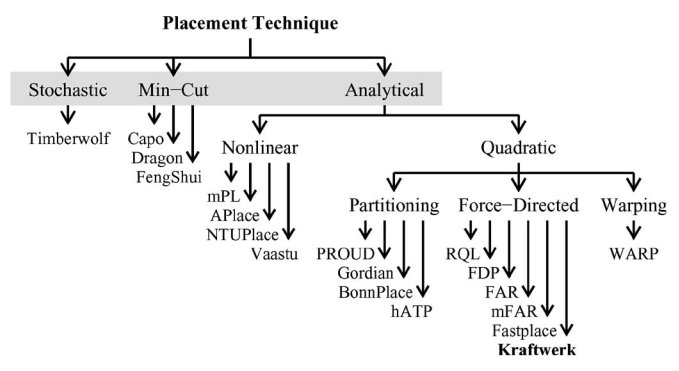
\includegraphics[width=0.75\textwidth]{figures/kraftwerk2.png}
        \end{center}
        \caption{Landscape of VLSI placement techniques (Spindler) \cite{kraftwerk2} }
        \label{fig:kraftwerk2}
    \end{figure}
    \begin{figure}
        \begin{center}
            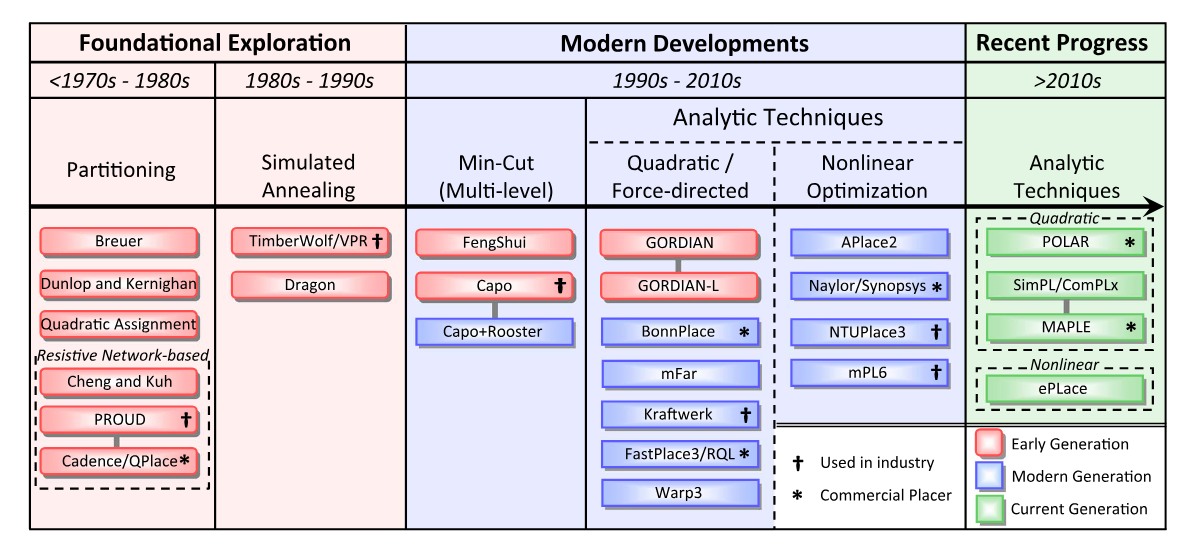
\includegraphics[width=0.95\textwidth]{figures/ProCha.png}
        \end{center}
        \caption{Historical timeline of VLSI placement techniques (Markov) \cite{ProCha} }
        \label{fig:ProCha}
    \end{figure}

    This is a citation for AMFPlacer. \cite{AMFPlacer}

    \newpage
    \bibliographystyle{ieeetr}
    \nocite{*}
    \bibliography{
        references/surveys,
        references/rapidwright,
        references/fpga_placement,
        references/vlsi_placement,
    }

\end{document}


